\documentclass[tikz]{standalone}

\begin{document}
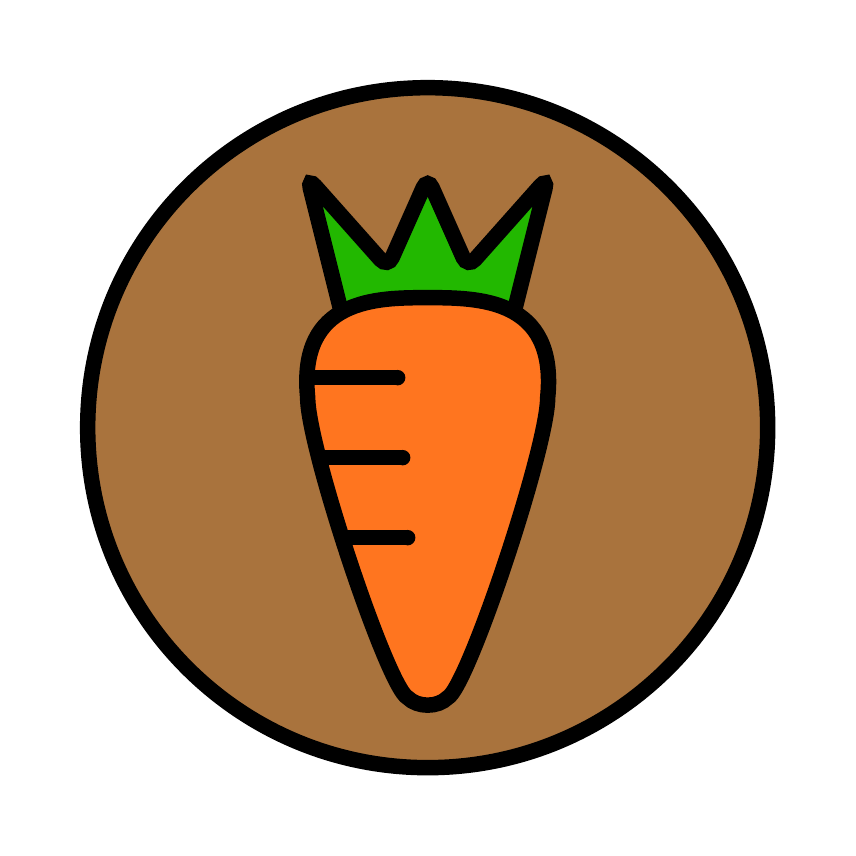
\begin{tikzpicture}[x=.5in, y=.5in]
  % Colors
  \definecolor{blank}{HTML}{ffffff}
  \definecolor{outline}{HTML}{000000}
  \definecolor{dirt}{HTML}{a9733d}
  \definecolor{stem}{HTML}{22b800}
  \definecolor{taproot}{HTML}{ff751f}

  % Configurations
  \tikzset{stroke/.style={line width=1.3ex, draw=#1}}

  % Drawing objects
  \newcommand{\stem}{%
    -- +(.8,0)
    -- +(1.2,1.6)
    -- +(.4,.7)
    -- +(0,1.6)
    -- +(-.4,.7)
    -- +(-1.2,1.6)
    -- +(-.8,0)
    -- cycle
  }
  \newcommand{\taproot}{%
    .. controls +(.5,0) and +(.1,1) .. +(1.2,-1)
    .. controls +(0,-.5) and +(.2,.1) .. +(.2,-4)
    .. controls +(-.1,-.1) and +(.1,-.1) .. +(-.2,-4)
    .. controls +(-.2,.1) and +(0,-.5) .. +(-1.2,-1)
    .. controls +(-.1,1) and +(-.5,0) .. cycle
  }

  % Bounding box
  \clip [rounded corners=1ex, preaction={fill=blank}]
  (0,0) rectangle (8,8);

  % Bounding circle
  \draw [fill=dirt] (4,4) circle (3.4);
  \draw [stroke] (4,4) circle (3.4);
  % Stem
  \draw [fill=stem] (4,4.9) \stem;
  \draw [stroke, rounded corners, draw=outline] (4,4.9) \stem;
  % Taproot
  \draw [fill=taproot] (4,5.3) \taproot;
  \draw [stroke, draw=outline] (4,5.3) \taproot;
  % Taproot lines
  \draw [stroke, rounded corners, draw=outline] (2.8,4.5) -- +(.9,0);
  \draw [fill=outline] (3.7,4.5) circle (.6ex);
  \draw [stroke, rounded corners, draw=outline] (2.9,3.7) -- +(.85,0);
  \draw [fill=outline] (3.75,3.7) circle (.6ex);
  \draw [stroke, rounded corners, draw=outline] (3.1,2.9) -- +(0.7,0);
  \draw [fill=outline] (3.8,2.9) circle (.6ex);
\end{tikzpicture}
\end{document}
